\documentclass[preprint,notitlepage]{revtex4-2}
\usepackage{amsmath, amssymb}
\usepackage{graphicx}
\usepackage{float}
\usepackage{booktabs}
\usepackage{xcolor}
\usepackage{tcolorbox}
\usepackage{hyperref}
\usepackage{enumitem}
\usepackage{physics}
\usepackage{caption}
\usepackage{bm}
\usepackage{tikz}
\usepackage{pgfplots}
\usepackage{lmodern}
\usepackage{amsmath,amssymb,amsfonts}
\usepackage{mathtools}
\usetikzlibrary{knots,intersections,decorations.pathreplacing}
\usetikzlibrary{3d, calc, arrows.meta, positioning}
\usepackage{pgfmath}
\usetikzlibrary{decorations.pathmorphing}
\pgfplotsset{compat=1.18} % or version you have
\usepackage{titlesec}
\usepackage{ulem}
\usepackage[utf8]{inputenc}
\usepackage[T1]{fontenc}
\renewcommand{\grqq}{``}


\begin{document}
\title{Revisiting the Æther:\\ From Einstein to the Vortex Fluid Paradigm}
\author{Omar Iskandarani\footnote{\scriptsize This paper is not intended as a neutral historical review, but as a conceptual bridge—framing the Vortex Æther Model (VAM) as a contemporary realization of Einstein’s late æther philosophy. \textbf{Keywords:} Æther, Einstein, Vortex fluid model, Time dilation, Topological gravity, Field theory, Helmholtz, Maxwell, Kelvin, unified field theory}}
\thanks{Independent Researcher, Groningen, The Netherlands\\
        info@omariskandarani.com \\
        ORCID: \href{https://orcid.org/0009-0006-1686-3961}{0009-0006-1686-3961} \\
        DOI: \href{https://doi.org/10.5281/zenodo.15669901}{10.5281/zenodo.15669901}}
\date{\today}
\maketitle

\begin{abstract}
This paper revisits the concept of the æther through Einstein’s post-1920 writings, culminating in a structured reinterpretation via the Vortex Æther Model (VAM). Contrary to the belief that Einstein abandoned the æther, we show that his later work restored it as a physically meaningful medium—devoid of mechanical motion but endowed with field-like properties essential for gravitation and inertia. We trace this shift from the 1905 rejection of the luminiferous æther to the 1924 Einstein–Cartan correspondence, emphasizing its continuity with modern field-theoretic frameworks.

VAM builds on this foundation by modeling the æther as an incompressible, inviscid superfluid. Gravitation and inertia emerge from the quantized circulation of knotted vortex filaments, with vorticity replacing curvature as the physical substrate of gravitational effects. Conserved angular momentum gives rise to time dilation, inertial response, and mass-energy equivalence. We define an effective mass profile \( M_{\text{eff}}(r) = \int_0^r 4\pi r'^2 \rho_\text{\ae}^{(\text{energy})}(r') \, dr' \), derived from localized vortex energy, and introduce a swirl potential \( \Omega(r) = \frac{C_e}{r_c} e^{-r/r_c} \), which governs fluid-mediated gravitation via Bernoulli-like pressure gradients.

Time dilation arises from tangential vortex flow as \( \frac{d\tau}{dt} = \sqrt{1 - \frac{v_\theta^2}{c^2}} \), with \( v_\theta(r) = \frac{\Gamma}{2\pi r} \), where \( \Gamma \) is the circulation quantum and \( v_\theta \) the local swirl velocity. This expression recovers relativistic time effects from fluid kinematics, without invoking curvature.

This sets a conceptual and mathematical foundation for VAM, in which classical and quantum behavior emerge from topological fluid dynamics. The model distinguishes three temporal modes within the æther: \( \mathcal{N} \) (Æther-Time), \( \tau \) (Proper Time), and \( S(t) = \int \Omega(r)\, dt \) (Swirl Clock Phase), offering a layered ontology of temporality. For empirical benchmarking against general relativity, see the companion analysis in~\cite{VAM-3}.
\end{abstract}


\section{Introduction}

It is often claimed that Einstein ``abolished the æther'' in his theory of relativity. While this has become a popular shorthand in both educational and philosophical discussions, it severely oversimplifies Einstein's actual position~\cite{einstein1920aether}. In his early work (1905), Einstein dispensed with the notion of the luminiferous æther as a mechanical carrier of electromagnetic waves. Yet, in later writings—most notably his 1920 lecture at Leiden—he reintroduced a more subtle concept of æther, reinterpreted within the context of spacetime geometry.
For historical quotations and their mappings to VAM dynamics, see Appendix~\ref{appendix:einstein}.


This paper revisits Einstein’s evolving perspective on the æther and evaluates its compatibility with the comprehensive Vortex Æther Model (VAM) program, as presented in the recent VAM master paper~\cite{VAM-8} and its companion studies. VAM proposes that the æther is a structured, incompressible fluid medium whose knotted vorticity fields underlie all known phenomena—gravitation, inertia, time, quantum behavior, and cosmological structure. Through a topological and dynamical synthesis, VAM provides not only a conceptual bridge but also explicit, testable predictions that unite historical field theory with contemporary advances in fundamental physics.~\cite{VAM-11, VAM-15}.

Unlike modern field theories that eliminate any underlying substrate, VAM embraces the æther as the unified, dynamically active fabric through which geometry, force, and phase propagate.

The goal of this study is twofold: first, to clarify Einstein’s nuanced philosophical stance regarding the æther—tracing its transformation from a mechanical substrate to a geometric and energetic foundation for field theory; and second, to construct a rigorous conceptual and mathematical bridge between this historical lineage and contemporary physics.

This bridge is now rendered concrete through the comprehensive VAM series (see ~\cite{VAM-8} for full derivations), which provides:

\begin{itemize}
    \item Explicit mathematical derivations of the foundational equations of VAM, including the emergence of gravitational, inertial, and quantum effects from topological swirl dynamics and the formal structure of multimodal time;
    \item A master equation for particle masses and a complete knot-based taxonomy, unifying leptons, baryons, and their quantum numbers (see Sec.~\ref{sec:taxonomy}, ~\cite{VAM-8}, ~\cite{VAM-11});
    \item Empirical benchmarking against classical and modern tests, as well as predictions for new phenomena in quantum gravity, cosmology, and particle physics (see ~\cite{VAM-8}, ~\cite{VAM-12}, ~\cite{VAM-15});
    \item A unified topological fluid-dynamical Lagrangian connecting all known interactions to a single underlying vortex æther (see ~\cite{VAM-14}).
\end{itemize}

Together, these advances transform the æther hypothesis from historical curiosity into a predictive, mathematically mature, and experimentally relevant framework for fundamental physics.

VAM now extends beyond gravity to encompass a unified, topological account of particle masses, quantum phenomena, and cosmology.

A historical overview of ætheral and vortex field theory—from Helmholtz to VAM—is provided in Appendices~\ref{appendix:helmholtz}–\ref{appendix:einstein}, alongside a mapping of Einstein’s quotations to the specific dynamical structures in VAM.

\vspace{1em}
\noindent\textbf{Lineage of Æther and Vortex Physics:}

\[\fbox{\makebox[2.2cm][c]{Helmholtz}} \;\longrightarrow\;\fbox{\makebox[2.2cm][c]{Kelvin}} \;\longrightarrow\;\fbox{\makebox[2.2cm][c]{Maxwell}} \;\longrightarrow\;\fbox{\makebox[2.2cm][c]{Einstein}} \;\longrightarrow\;\fbox{\makebox[2.2cm][c]{VAM}}\]

\begin{center}
\scriptsize
\textit{
Conservation of vorticity $\;\rightarrow\;$ Topological atoms $\;\rightarrow\;$ Field stress in æther $\;\rightarrow\;$ Geometric æther $\;\rightarrow\;$ Unified Vortex-fields
}
\end{center}
% Equal-width date boxes
\[\fbox{\makebox[2.2cm][c]{(1858)}} \;\longrightarrow\;\fbox{\makebox[2.2cm][c]{(1867--1890)}} \;\longrightarrow\;\fbox{\makebox[2.2cm][c]{(1875--1878)}} \;\longrightarrow\;\fbox{\makebox[2.2cm][c]{(1920--1924)}} \;\longrightarrow\;\fbox{\makebox[2.2cm][c]{(2012--2025)}}\]

\vspace{1em}
\section{Reevaluating Einstein’s Supposed Rejection of the Æther}

Einstein’s 1905 formulation of Special Relativity omitted the luminiferous æther as a mechanical necessity for light propagation. This has often been misinterpreted as a categorical rejection of any æther concept. However, Einstein’s statement was more nuanced:
\begin{quote}
    ``The introduction of a 'light-bearer' æther proves to be superfluous.''
\end{quote}

This does not deny the possibility that space possesses structure or physical attributes. Instead, it marks a shift from a mechanical to a field-theoretic perspective, not an ontological negation of any spacetime substrate. As explored in Section~\ref{sec:einstein_aether}, Einstein would later revisit and explicitly refine the æther concept in the context of General Relativity.

This perspective—where space retains structure but not particulate substance—prefigures the modern VAM approach, in which the æther is formalized as a quantized, topological superfluid (see Sec.~\ref{sec:VAM_overview}, and~\cite{VAM-8}).

\section{The Return of the Æther Concept (1920)}

Einstein’s 1920 Leiden lecture marks a critical clarification:
\begin{quote}
    ``According to the general theory of relativity, space is endowed with physical qualities; in this sense, therefore, there exists an æther. According to the general theory of relativity, space without æther is unthinkable.''~\cite{einstein1920aether}
\end{quote}

In this revised conception, the æther is not a mechanical substance but a geometric and energetic substrate. It carries properties such as curvature, stress-energy, and gravitational potential, and is inseparable from the fabric of spacetime. This evolution in Einstein’s thought forms the philosophical foundation for VAM, which regards the æther as a structured, dynamically active fluid rather than an inert void~\cite{VAM-8}.

In what follows, we examine Einstein’s later writings in this light and develop a fluid-dynamical continuation of his geometric intuition—now realized as a quantized, topologically rich superfluid with explicit links to particle physics and cosmology.

\section{Æther as Carrier of Field Quality}

Einstein explicitly redefined the æther in his later writings as a non-material but physically active entity. He emphasized that this æther:
\begin{itemize}
    \item Not composed of discrete particles,
    \item Not endowed with a state of absolute rest,
    \item Yet responsible for observable effects such as gravitation, field propagation, and the progression of time.
\end{itemize}

This interpretation departs from the 19th-century particulate æther, aligning instead with a modern view of the vacuum as a continuous, structured background. The VAM framework adopts this perspective, modeling space as a (nearly) incompressible, inviscid superfluid in which all forces, fields, and even quantum phenomena emerge from topologically conserved vorticity and structured swirl~\cite{VAM-8, VAM-1, VAM-2}.

\vspace{0.7em}
\noindent\textbf{Recent Results:}
Mathematically, these ideas are realized in VAM by:
\begin{itemize}
    \item Explicit definitions of absolute time (\(\boldsymbol{\mathcal{N}}\)), proper time (\(\boldsymbol{\tau}\)), and internal phase clocks (\(\boldsymbol{S}^{\boldsymbol{\circlearrowleft}}_\text{(t)}\)), as rigorously formulated in~\cite{VAM-8, VAM-1}.
    \item Derivation of gravitational and inertial effects from swirl-induced pressure gradients, replacing geometric curvature in General Relativity (see~\cite{VAM-2, VAM-3, VAM-8}).
    \item A master mass equation relating particle rest masses to vortex topology, and a complete knot taxonomy for all Standard Model particles~\cite{VAM-8, VAM-11}.
    \item Direct empirical benchmarking of VAM predictions for time dilation, redshift, frame-dragging, and cosmological phenomena (see~\cite{VAM-3, VAM-8}).
    \item Formulation of a unified topological Lagrangian encompassing all known interactions (see~\cite{VAM-14}).
\end{itemize}

In this view, the metric tensor and curvature of GR become emergent, large-scale approximations of the underlying vortex field dynamics—a hypothesis now rendered testable and falsifiable through precise mathematical and observational correspondence (see Sections~\ref{sec:benchmarking}–\ref{sec:lorentz_recovery}, and~\cite{VAM-8}).

\vspace{0.8em}
\noindent\textbf{Ætheric Temporal Sequence:}
\begin{center}
\(\boldsymbol{\mathcal{N}} \to \boldsymbol{\nu_0} \to \boldsymbol{\tau} \to \boldsymbol{S}^{\boldsymbol{\circlearrowleft}}_\text{(t)} \to \boldsymbol{T_v} \to \mathbb{\boldsymbol{K}}\)
\end{center}

\section{Multimodal Time: The Ætheric Temporal Ontology}

The Vortex Æther Model (VAM) advances a multimodal conception of time, rooted in the internal and relational dynamics of an incompressible, inviscid æther. Unlike the unidimensional time parameter in standard field theory or the proper time of General Relativity, VAM’s temporal taxonomy encapsulates distinct physical, topological, and informational modes, each with a clear analytical and experimental role. This layered approach not only extends Einstein’s “geometric æther” but also provides a framework for modeling causality, memory, and quantum-classical transitions in a unified manner~\cite{VAM-8, VAM-13, VAM-15}.

The multimodal temporal ontology of VAM is not purely an abstract taxonomy; it possesses a geometric and topological structure, naturally visualized as a multidimensional “spiral” or “fan” in phase space (see Fig.~\ref{fig:temporal_ontology}). Each temporal mode—Aithēr-Time, Now-Point, Chronos-Time, Swirl Clock, Vortex Proper Time, and Kairos Moment—plays an independent yet interconnected role, governing different layers of physical law~\cite{VAM-8, VAM-13}.

\begin{figure}[H]
    \centering
    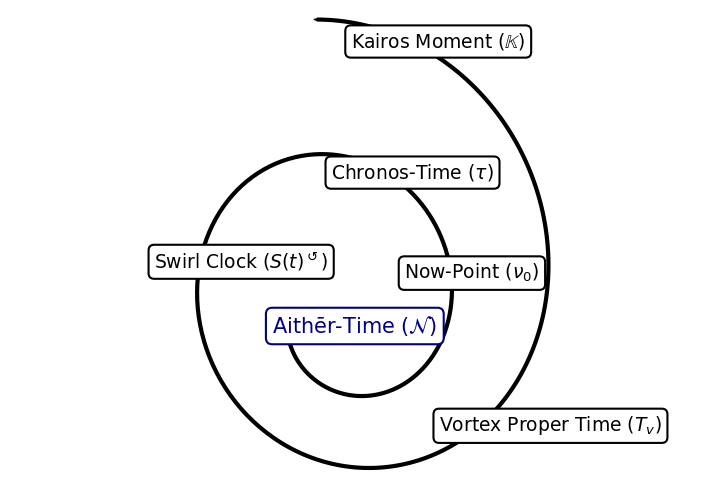
\includegraphics[width=0.7\textwidth]{TemporalOntology}
    \caption{
        \textbf{Vortex Phase Spiral of Ætheric Time.}
        The sequential emergence of time modes in the VAM ontology, proceeding outward from the core of Aithēr-Time ($\boldsymbol{\mathcal{N}}$), through Now-Point ($\boldsymbol{\nu_0}$), Chronos-Time ($\boldsymbol{\tau}$), Swirl Clock ($\boldsymbol{S}^{\boldsymbol{\circlearrowleft}}_\text{(t)}$), Vortex Proper Time ($\boldsymbol{T_v}$), to the outermost Kairos Moment ($\mathbb{\boldsymbol{K}}$). Each layer represents a distinct analytical and physical role, together forming a unified temporal architecture underlying vortex dynamics~\cite{VAM-8, VAM-13}.
    }
    \label{fig:temporal_ontology}
\end{figure}

\begin{tcolorbox}[
  colback=gray!10,
  colframe=black,
  width=0.9\textwidth,
  sharp corners=southwest,
  boxrule=0.5pt,
  before skip=10pt,
  after skip=10pt,
  title=\textbf{Table: Ætheric Time Modes in the Vortex Æther Model},
  fonttitle=\bfseries,
]
\renewcommand{\arraystretch}{1.25}
\small
\begin{tabular}{r l l}
  $\boldsymbol{\mathcal{N}}$     & \textbf{Aithēr-Time}         & Absolute causal ordering parameter~\cite{VAM-8, VAM-13} \\
  $\boldsymbol{\nu_0}$           & \textbf{Now-Point}           & Localized intersection with universal present~\cite{VAM-8, VAM-13} \\
  $\boldsymbol{\tau}$            & \textbf{Chronos-Time}        & Measurable time in the æther (subject to dilation)~\cite{VAM-1, VAM-8} \\
  $\boldsymbol{S}^{\boldsymbol{\circlearrowleft}}_\text{(t)}$ & \textbf{Swirl Clock}         & Internal phase memory of a vortex~\cite{VAM-2, VAM-13, VAM-15} \\
  $\boldsymbol{T_v}$             & \textbf{Vortex Proper Time}  & Circulation-based geodesic duration~\cite{VAM-2, VAM-13} \\
  $\mathbb{\boldsymbol{K}}$      & \textbf{Kairos Moment}       & Discrete topological bifurcation event~\cite{VAM-13, VAM-15} \\
\end{tabular}
\end{tcolorbox}

\noindent The interpretation of each mode is as follows:
\begin{itemize}
    \item \textbf{Aithēr-Time ($\boldsymbol{\mathcal{N}}$):} The unobservable but indispensable global time parameter that orders all events causally within the ætheric manifold, serving as the absolute temporal background for physical processes~\cite{VAM-8, VAM-13}.

    \item \textbf{Now-Point ($\boldsymbol{\nu_0}$):} The localized realization of the present, defined by the intersection of the global time field $\boldsymbol{\mathcal{N}}$ with a point in the æther manifold. It establishes the surface of simultaneity and facilitates causal foliation~\cite{VAM-8, VAM-13}.

    \item \textbf{Chronos-Time ($\boldsymbol{\tau}$):} The physically measurable flow of time, experienced within the æther and modulated by local vorticity through swirl-induced time dilation~\cite{VAM-1, VAM-8}:
    \[
        \frac{d\boldsymbol{\tau}}{dt} = \sqrt{1 - \boldsymbol{v_\phi}^2(r)/c^2}
    \]
    where $\boldsymbol{v_\phi}(r)$ is the local tangential velocity of the vortex field.

    \item \textbf{Swirl Clock ($\boldsymbol{S}^{\boldsymbol{\circlearrowleft}}_\text{(t)}$):} The internal phase variable of a vortex structure, tracking angular displacement and serving as a memory function for topological identity and history. It is formally given by~\cite{VAM-2, VAM-13}:
    \[
        \boldsymbol{S}^{\boldsymbol{\circlearrowleft}}_\text{(t)} = \int_{0}^{t} \boldsymbol{\Omega}(r(t'))\, dt'
    \]
    with $\boldsymbol{\Omega}(r)$ the local angular velocity.

    \item \textbf{Vortex Proper Time ($\boldsymbol{T_v}$):} The intrinsic circulation-based duration associated with a closed path around a vortex core, defined as~\cite{VAM-2, VAM-13}
    \[
        \boldsymbol{T_v} = \oint \frac{dl}{\boldsymbol{v_\phi}(r)}
    \]
    representing the intrinsic “clock” of a knotted structure.

    \item \textbf{Kairos Moment ($\mathbb{\boldsymbol{K}}$):}
    The discrete event marking a topological transition such as vortex reconnection or bifurcation, producing an irreversible change in vortex identity and introducing discontinuities or non-analyticities in the evolution of $\boldsymbol{T_v}$ or $\boldsymbol{S}^{\boldsymbol{\circlearrowleft}}_\text{(t)}$~\cite{VAM-13, VAM-15}.
\end{itemize}

In the VAM framework, the “Kairos Moment” ($\mathbb{\boldsymbol{K}}$) represents a discrete, topologically induced transition in the evolution of vortex matter—such as a vortex reconnection, bifurcation, or the passage of a gravitational wave. These events break the smooth evolution of the Swirl Clock phase and manifest as quantized phase slips or time jumps. As shown in Fig.~\ref{fig:kairos_moment}, a Kairos event appears as an abrupt change in the Swirl Clock trajectory during a localized temporal window. Such phenomena are experimentally accessible in analog systems and may be detectable in astrophysical settings as phase anomalies or decoherence events in quantum or classical fields~\cite{VAM-13, VAM-15}.

\begin{figure}[H]
    \centering
    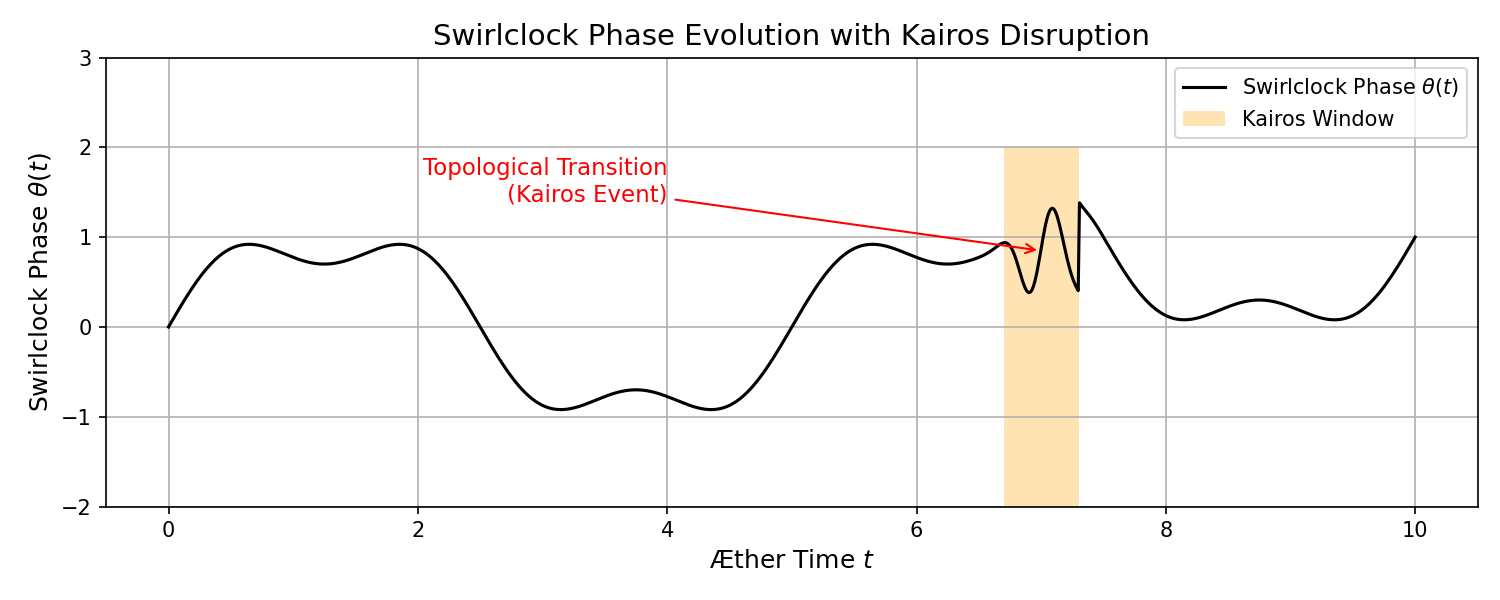
\includegraphics[width=0.7\textwidth]{TemporalOntologyKairosMoment}
    \caption{
        \textbf{Swirlclock Phase Evolution with Kairos Disruption.}
        The evolution of the Swirl Clock phase, $\theta(t)$, as a function of Æther Time ($t$), illustrating a topological transition (“Kairos Event”) as a discontinuity in the phase trajectory. The highlighted “Kairos Window” denotes the temporal interval where a critical event (such as vortex reconnection or a passing gravitational wave) induces an irreversible shift or decoherence in the internal phase. Such events correspond to the “Kairos Moment” ($\mathbb{\boldsymbol{K}}$) in the VAM temporal ontology, marking the transition from smooth, memory-preserving evolution to a new dynamical regime. This demonstrates how topological or energetic disruptions in the æther manifest as observable time “jumps” or phase slips in physical systems~\cite{VAM-13, VAM-15}.
    }
    \label{fig:kairos_moment}
\end{figure}

This multimodal temporal ontology enables VAM to bridge metaphysical continuity with physically testable vortex dynamics. It underpins several core applications in the extended VAM literature, including models of causality, gravitational time dilation, vortex identity, and swirl-induced phase decoherence~\cite{VAM-1, VAM-2, VAM-8, VAM-13, VAM-15}. For detailed derivations, see~\cite{VAM-2, VAM-8, VAM-13, VAM-15}.

\section{Connection to the Vortex Æther Model (VAM)}

The Vortex Æther Model (VAM), developed by O. Iskandarani since 2012, models the æther as an incompressible, non-viscous superfluid~\cite{VAM-8, VAM-13}. Within this framework, vorticity is elevated to a fundamental quantity that governs time dilation, inertial mass, and gravitational interaction~\cite{VAM-2, VAM-10, VAM-13}. Echoing Einstein’s 1920 redefinition of the æther as a physical substratum, VAM treats the æther as a structured, causal medium from which all dynamical behavior emerges~\cite{VAM-8}.

Key structural elements of VAM include:
\begin{itemize}
    \item \textbf{Topological structures} (e.g., knots, trefoils) representing stable particle identities and quantum numbers~\cite{VAM-8, VAM-11, VAM-14},
    \item \textbf{Time dilation} arising from swirl intensity near vortex cores~\cite{VAM-2, VAM-13},
    \item \textbf{A revised system of natural constants}, including $C_e$ (vortex boundary velocity) and $F^{\max}_{\text{\ae}}$ (maximum ætheric stress), defined and operationalized in the topological Lagrangian~\cite{VAM-14}.
\end{itemize}

\subsection*{VAM-Derived Expression for $\boldsymbol{G}$}

One of the notable results in VAM is a derivation of the gravitational constant in terms of ætheric and topological parameters~\cite{VAM-2, VAM-13, VAM-14}. Rewriting the expression in dimensionally transparent form:

\begin{equation}
    G_\text{swirl} = \frac{C_e}{2 F^{\max}_{\text{\ae}}} \cdot \left( \frac{c^5 t_p^2}{r_c^2} \right)
\end{equation}

\noindent where:
\begin{itemize}
    \item $C_e$: swirl velocity at the vortex boundary (m/s),
    \item $F^{\max}_{\text{\ae}}$: maximum force the æther can sustain before bifurcation (N),
    \item $t_p$: Planck time $ \left(\sqrt{\hbar G / c^5}\right) $,
    \item $r_c$: core radius of the vortex structure (m),
    \item $c$: speed of light in vacuum (m/s).
\end{itemize}

This formulation emerges from the Swirl Clock formalism and connects gravity to rotational energy density under conservation of circulation~\cite{VAM-2, VAM-13}. It expresses $G$ not as a fundamental input constant, but as a derived quantity arising from the interplay of topological scale $r_c$, rotational dynamics $C_e$, and ætheric tension $F^{\max}_{\text{\ae}}$. This reinforces the view that gravitation is a residual effect of conserved vorticity in a compressible ætheric medium.

VAM further incorporates circulation quantization, helicity conservation, and pressure-mediated interactions to model the exchange between knotted structures and their surrounding swirl fields~\cite{VAM-8, VAM-11, VAM-14}. This general framework aligns with Einstein’s late attempt at a unified field theory—now realized through the mathematics of topological fluid dynamics.

The model's predictions are experimentally approachable through analog systems such as rotating superfluid vortices, BEC interference patterns, and refractive index shifts under swirl acceleration~\cite{VAM-2, VAM-13}. These offer testable pathways for validating the core dynamics proposed by VAM.

\vspace{1em}

\section{Historical Continuity and Outlook}

A careful reexamination of Einstein's later writings reveals that he:
\begin{itemize}
    \item Did \emph{not} reject the æther outright, but \emph{redefined} it as a field-carrying substrate~\cite{einstein1920aether},
    \item Sought a \textbf{continuous medium} bearing the properties of spacetime without requiring mechanical motion,
    \item And ultimately pursued a \textbf{unified field theory}—one that VAM now echoes through the interplay of gravity, time perception, and vorticity~\cite{VAM-8, VAM-14}.
\end{itemize}

Einstein recognized that space could not be entirely void—it had to possess structural, energetic, and causal qualities. In this context, the Vortex Æther Model is not a speculative throwback, but a mathematically grounded continuation of Einstein's vision. It operationalizes this active structure via conserved vortex fields, topological knot invariants, and energy-sustaining boundary flows~\cite{VAM-8, VAM-11, VAM-14}.

While other contemporary models—such as emergent gravity and superfluid vacuum theory—have gestured toward similar foundations, VAM distinguishes itself by offering an explicitly solvable, hydrodynamically derived, and testable framework~\cite{VAM-8, VAM-14, VAM-15}. It bridges general relativity, thermodynamics, and quantum field heuristics without requiring discrete particles or quantized spacetime.

Kelvin's concern regarding topological degeneracy is addressed in Appendix~\ref{appendix:kelvin}.


\section*{Conclusion and Forward Outlook: Æther Reclaimed}

Modern theoretical physics is gradually converging on insights once considered obsolete—not because the underlying concepts were invalid, but because earlier mathematical and experimental tools lacked the necessary precision. Einstein’s late-career perspective on the æther anticipated this renaissance: a vision of space as a continuous, energetic, and causally structured medium. The Vortex Æther Model (VAM) builds directly on this foundation, advancing it into a unified, predictive, and testable framework~\cite{VAM-8, VAM-13, VAM-14}.

Here, vorticity and topological structure supplant the classical notion of curvature, and time itself emerges as a hierarchy of circulation and phase—fully realized in the multimodal temporal ontology~\cite{VAM-13, VAM-15}. The æther, once dismissed, returns in a new form: not as a mechanical ether, but as a quantized, causal, and observable substrate underlying all known phenomena—from gravitation and particle masses to quantum measurement and cosmological evolution~\cite{VAM-8, VAM-11, VAM-15}.

VAM does not merely offer a philosophical bridge to Einstein’s “unified field” dream, but delivers a rigorous technical foundation and explicit predictions that now invite empirical validation. With advancing experiments in superfluid analogues, quantum vortex interferometry, and photonic swirl, the opportunity to test, refine, or falsify these ideas moves within experimental reach~\cite{VAM-2, VAM-13, VAM-15}.

It is time to move beyond the view of Einstein as the man who abolished the æther, and instead to recognize him as the thinker who quietly reframed it—preparing the ground for its scientific rebirth. In that spirit, the Vortex Æther Model is not a closure, but an opening: a dynamic, empirically accessible, and mathematically coherent path forward in the ongoing quest for a unified physical theory.

\subsection*{Future Directions and Experimental Signatures}

The path forward for the Vortex Æther Model is both theoretically rich and experimentally accessible. On the theoretical front, continued development will further refine the topological classification of particle states~\cite{VAM-11, VAM-14}, explore fractal swirl dynamics at both quantum and cosmological scales~\cite{VAM-12, VAM-9}, and formalize the mechanisms by which gravitation and quantum phenomena emerge from circulation and helicity conservation~\cite{VAM-13, VAM-15}.

Empirically, the VAM framework provides several concrete predictions and signatures amenable to near-future tests:
\begin{itemize}
    \item \textbf{Time dilation and frame-dragging effects} in laboratory superfluids, Bose–Einstein condensates, and photonic vortex lattices~\cite{VAM-2, VAM-13};
    \item \textbf{Swirl clock phase slips and Kairos events} observable as quantized phase jumps or decoherence in quantum vortex interferometry~\cite{VAM-15};
    \item \textbf{Anomalous redshift, light bending, and perihelion precession} in astrophysical observations that deviate from standard General Relativity in high-vorticity or topologically complex environments~\cite{VAM-10};
    \item \textbf{Spectral and mass predictions} for leptons, baryons, and their excited states, determined by knot topology and quantized circulation~\cite{VAM-11, VAM-14};
    \item \textbf{Novel cosmological signatures} arising from large-scale swirl structure and the fractal dynamics of the æther, potentially visible in galaxy rotation curves and the cosmic microwave background~\cite{VAM-9, VAM-12}.
\end{itemize}

By combining theoretical coherence with falsifiable experimental predictions, the Vortex Æther Model opens a concrete research agenda for unifying gravitation, quantum mechanics, and cosmology. As the boundaries of precision measurement and analog simulation continue to expand, VAM stands poised to guide and interpret the next wave of discoveries at the intersection of topology, fluid dynamics, and fundamental physics.



\appendix
\section*{Appendix I: Helmholtz and the Foundations of Vortex Physics}
\label{appendix:helmholtz}
\addcontentsline{toc}{section}{Appendix I: Helmholtz on Vorticity}

    Hermann von Helmholtz’s 1858 paper \textit{“On the Integrals of the Hydrodynamic Equations Corresponding to Vortex Motion”}~\cite{helmholtz1858vortices} marks the formal beginning of vortex theory in physics. His theorems define the behavior of vorticity in an ideal, incompressible fluid—concepts foundational to the Vortex Æther Model (VAM).

    \subsection*{1. Vorticity is conserved along fluid lines}
    \begin{quote}
    \textit{“Each portion of a vortex filament remains connected to the same fluid elements throughout the motion.”}
    \end{quote}

    \textbf{VAM Mapping:} This becomes the core of VAM’s knot stability. Swirl identity is maintained via conserved helicity and circulation:
    \[
    \frac{d\Gamma}{dt} = 0, \quad \Gamma = \oint_{\mathcal{C}} \vec{v} \cdot d\vec{\ell}
    \]

    \subsection*{2. Vortex lines cannot end in a fluid — they form closed loops or extend to boundaries}
    \begin{quote}
    \textit{“The extremities of a vortex line cannot exist within the fluid; they must lie at the boundaries or form closed curves.”}
    \end{quote}

    \textbf{VAM Mapping:} Explains the closed-loop structure of particle-knot analogues in VAM. Vortices are topologically confined:
    \[
    \nabla \cdot \vec{\omega} = 0
    \]

    \subsection*{3. Circulation is invariant under ideal flow}
    \begin{quote}
    \textit{“The circulation around a closed curve moving with the fluid remains constant.”}
    \end{quote}

    \textbf{VAM Mapping:} VAM uses this to define internal clocks, mass, and swirl energy. This law becomes the origin of the time dilation formula:
    \[
    S(t) = \int \omega(t) \, dt, \quad T_v \sim \Gamma^{-1}
    \]

    \subsection*{Historical Legacy}

    Helmholtz's influence extended deeply into Kelvin’s vortex atom theory, Maxwell’s mechanical æther models, and later Einsteinian field theory. Today, in the Vortex Æther Model, his principles live on as conservation laws that define both structure and evolution of the physical vacuum.

    \begin{quote}
    \textit{“If matter is vortex, then Helmholtz is its first architect.”}
    \end{quote}
   \hfill — O. Iskandarani

\section*{Appendix II: Lord Kelvin and the Knot-Æther Critique}
\addcontentsline{toc}{section}{Appendix II: Lord Kelvin}
\label{appendix:kelvin}

    In the late 19th century, William Thomson (Lord Kelvin) proposed that atoms might be stable vortex knots in an invisible æther — a topological interpretation of matter. Yet he himself raised the most pointed critique:

    \begin{quote}
    \("\) I am afraid of the smoke and complication, of all the varieties of knots and links, if they are to explain the variety of elements.\("\)
    \end{quote}
 \hfill  — Lord Kelvin, 1890

    Kelvin feared that the near-infinite number of possible knots and links in three-dimensional space would not correspond to the relatively small number of stable chemical elements~\cite{thomson1890knots, tait1877knots}. Without a natural principle of selection, the theory risked degeneracy: the proliferation of mathematically possible but physically irrelevant structures.

    \subsection*{Historical Context}

    In the second half of the 19th century, the vortex atom theory was developed, primarily by William Thomson (Lord Kelvin) and Peter Guthrie Tait~\cite{thomson1890knots, tait1877knots}. In this framework, atoms were envisioned as stable knots or vortex rings in an ideal, invisible fluid — the so-called luminiferous æther. The idea was that both the discrete nature of atomic species and their remarkable stability could be explained through topological invariants from knot theory.

    Helmholtz's 1858 paper introduced the conservation of vorticity in ideal fluids, laying the mathematical foundation upon which Kelvin and Tait constructed the vortex atom theory~\cite{helmholtz1858vortices}. This conservation principle is central to both classical vortex stability and the topological persistence employed in VAM.

    Kelvin's model was deeply influenced by the work of Helmholtz (1858) on vortex conservation in ideal fluids. He imagined that different types of knotted or linked vortices might correspond to different elements.

    \subsection*{Kelvin's Principal Objection}

    Despite its elegance, Kelvin identified a critical flaw:

    \begin{quote}
    \("\) I am afraid of the smoke and complication, of all the varieties of knots and links, if they are to explain the variety of elements.\("\)
    \end{quote}\\
     \hfill — William Thomson (Lord Kelvin), Baltimore Lectures, 1890\\
    The mathematical space of knots is vast, and Kelvin recognized the absence of a physical filter. He was acutely aware that the theory, though geometrically rich, lacked a way to explain *why only some knots should be stable atoms*. It had no built-in energetic, dynamic, or entropic selection rule.

    \subsection*{Experimental Shortcomings}

    Kelvin also noted the absence of empirical correspondence between specific knot types and actual elements. Without experimental access to the supposed vortex knots — their formation, stability, or interaction — the theory remained speculative.

    Nonetheless, the idea lived on, inspiring both topological mathematics and future models of discrete matter arising from continuous media.

    \subsection*{Comparison to the Modern Particle Zoo}

    Kelvin's critique is echoed in modern particle physics. The Standard Model contains a large number of particles, generations, couplings, and constants — many set only by experimental input, not derivable from deeper principles.

    \begin{quote}
    \textit{\("\) I am afraid I must end by saying that the difficulties are so great in the way of forming anything like a comprehensive theory, that we cannot even imagine a finger-post pointing to a way that leads us towards the explanation.} \\
    \textit{But this time next year — this time ten years — this time one hundred years — I cannot doubt but that these things which now seem to us so mysterious will be no mysteries at all. The scales will fall from our eyes. We shall learn to look on things in a different way — when that which is now a difficulty will be the only common-sense and intelligible way of looking at the subject.\("\)}
    \end{quote}
    \hfill — *Lord Kelvin, circa 1889*

    The degeneracy Kelvin foresaw reappears: a theory with many admissible but unexplained types of particles. The need for a *selection mechanism* remains urgent.

    \subsection*{The VAM Response}

    The Vortex Æther Model (VAM) revives the topological atom intuition but answers Kelvin's critique with concrete physical principles:

    \begin{itemize}
      \item Thermodynamic constraints (via Clausius entropy) limit allowable knot growth~\cite{clausius1865entropy}.
      \item Quantized circulation excludes unstable, high-energy configurations.
      \item Absolute vorticity conservation enforces topological stability.
      \item Vortex reconnection thresholds act as evolutionary boundaries.
    \end{itemize}

    As a result, VAM predicts only a finite, physically meaningful spectrum of topological matter structures — in line with observed baryons and leptons.

    \subsection*{Concluding Reflection}

    Kelvin's objection was not to knots themselves, but to their uncontrolled proliferation. VAM reclaims his vision, but grounds it in hydrodynamic logic, energy bounds, and field evolution:

    \begin{quote}
     \("\) Knots without constraints become chaos. Knots with physics become atoms.\("\)
    \end{quote}
   \hfill — O. Iskandarani

\section*{Appendix III: James Clerk Maxwell on the Æther and the Vortex Atom Theory}
\addcontentsline{toc}{section}{Appendix III: James Clerk Maxwell on the Æther and the Vortex Atom Theory}
\label{appendix:maxwell}

    James Clerk Maxwell (1831–1879), one of the foundational figures of modern physics, held deep and evolving views on the concept of the æther. While best known for formulating the electromagnetic field equations, Maxwell also contributed to the theoretical underpinnings of the æther and engaged directly with the emerging vortex atom theories of his time.

    \subsection*{Maxwell's View on the Æther}
    Maxwell firmly believed that the æther was a physically real, omnipresent medium necessary for the transmission of electromagnetic waves~\cite{maxwell1878britannica}:

    \begin{quote}
    \("\)There can be no doubt that the interplanetary and interstellar spaces are not empty, but are occupied by a material substance\ldots which is certainly the largest and probably the most uniform body of which we have any knowledge.\("\)
    \end{quote}

    To Maxwell, the electromagnetic field was not abstract, but a manifestation of real stresses and strains in the æther~\cite{maxwell1878britannica}. He imagined it as an elastic medium capable of supporting tension (electric fields), rotation (magnetic lines), and vibrational energy (light).

    \subsection*{Maxwell and the Vortex Atom Theory}

    Maxwell was intrigued by Lord Kelvin's proposal that atoms could be modeled as stable vortex knots in the æther — the so-called vortex atom theory~\cite{maxwell1875molecules}. In his 1875 lecture \("\)Molecules,\("\) he expressed qualified enthusiasm:

    \begin{quote}
    \("\)The vortex theory of atoms, first proposed by Helmholtz and developed by Sir William Thomson\ldots has made it conceivable that the properties of matter may depend solely on motion in a medium, and not on anything in the nature of the atom itself.\("\)
    \end{quote}
   \hfill — James Clerk Maxwell, 1875, \("\)Molecules\("\)

    This radical idea — that all matter could emerge from organized motion in a universal fluid — deeply appealed to Maxwell's mechanical sensibilities. However, he also expressed caution:

    \begin{quote}
    \("\)The difficulty is that we know so little about fluid motion, and the equations are so intractable, that no one has yet been able to deduce the properties of any known substance from such a theory.\("\)
    \end{quote}

    In short, the theory was conceptually beautiful but lacked mathematical tractability and predictive power. Maxwell understood the elegance of vortex-based models but noted that fluid dynamics was still too undeveloped to make the theory physically useful~\cite{maxwell1875molecules}.

    \subsection*{Legacy and Connection to VAM}

    Maxwell's æther was a mechanical medium filled with stresses, pressures, and circulations — not unlike the vortex fields described in the Vortex Æther Model (VAM). His aspirations for a unified field theory based on æther mechanics resonate strongly with VAM's goals:

    \begin{itemize}
      \item Both view the vacuum as structured and dynamic.
      \item Both describe matter as emergent from motion in the medium.
      \item Both seek to replace ad hoc constants with field-based origins.
    \end{itemize}

    Maxwell anticipated that future physicists might unlock the mathematics of vortex-structured æther. VAM — using conservation of vorticity, topological invariants, and pressure-induced time dilation — picks up where Maxwell's generation left off.

    \subsection*{Reflection}

    Maxwell's words remind us that the æther was never fully dismissed on scientific grounds, but rather due to limitations in modeling and experiment. With modern tools, those limitations are no longer insurmountable.

    \begin{quote}
    \textit{"A field is not a ghost. It is the visible strain of the invisible æther."}
    \end{quote}
    \hfill  — paraphrased from Maxwell's writings


\section*{Appendix IV: Einstein on the Æther — Translated Quotes and VAM Equivalents}
\addcontentsline{toc}{section}{Appendix IV: Einstein on the Æther}
\label{appendix:einstein}

    This appendix collects and annotates key statements made by Albert Einstein about the æther, focusing especially on how these statements align or contrast with the structure and assumptions of the Vortex Æther Model (VAM). Where possible, original German excerpts are included, with English translations and a mapping to VAM concepts or equations.

    \subsection*{1. \grqq Der Raum ohne Äther ist undenkbar...\textquotedblright}
    \textbf{Original (1920 Leiden Lecture):} \\
    \("\)Nach der allgemeinen Relativitätstheorie ist der Raum mit physikalischen Eigenschaften begabt; in diesem Sinne existiert also ein Äther. Gemäß der allgemeinen Relativitätstheorie ist ein Raum ohne Äther undenkbar.\("\)

    \textbf{Translation:} \\
    \("\)According to the general theory of relativity, space is endowed with physical qualities; in this sense, therefore, there exists an æther. According to the general theory of relativity, space without æther is unthinkable.\("\)

    \textbf{VAM Mapping:} \\
    This matches VAM's foundational postulate that the æther is a structured, non-viscous, incompressible medium with internal physical dynamics. The VAM equivalent is the existence of a vorticity-carrying background field \( \vec{\omega}(\vec{r}, t) \), subject to conservation laws and boundary conditions.

    \[
    \nabla \cdot \vec{v} = 0, \quad \nabla \cdot \vec{\omega} = 0, \quad \partial_t \vec{\omega} + (\vec{v} \cdot \nabla) \vec{\omega} = (\vec{\omega} \cdot \nabla) \vec{v}
    \]

    \subsection*{2. \grqq Es scheint, als sei die Einführung eines Äthers überflüssig...\textquotedblright}
    \textbf{Original (1905, SR paper):} \\
    \("\)Es scheint, als sei die Einführung eines Äthers überflüssig, insofern die Lichtausbreitung durch Maxwell'sche Gleichungen in leerem Raum ausreichend beschrieben werden kann.\("\)

    \textbf{Translation:} \\
    \("\)It seems that the introduction of an æther is superfluous, insofar as the propagation of light can be described adequately by Maxwell's equations in vacuum.\("\)

    \textbf{VAM Mapping:} \\
    Einstein's 1905 view was contextually specific to the Maxwellian field theory. VAM expands this to a \emph{sub-Maxwellian} fluid substrate: the fields emerge from vortex dynamics.

    VAM introduces: \\
    \( \vec{E} = -\nabla \Phi - \partial_t \vec{A}, \quad \vec{B} = \nabla \times \vec{A} \) as secondary fields derived from swirl-based potentials in the æther.

    \subsection*{3. \grqq Der Äther darf nicht als ein Medium mit mechanischen Eigenschaften gedacht werden...\textquotedblright}
    \textbf{Original (1920):} \\
    \("\)Der Äther darf nicht als ein Medium mit mechanischen Eigenschaften gedacht werden, wie es die alten Ätherkonzepte vorschlugen. Er besitzt keine Bewegungen, wie z.B. Geschwindigkeit.\("\)

    \textbf{Translation:} \\
    \("\)The æther must not be thought of as a medium with mechanical properties, as the old concepts of æther suggested. It has no motion in the usual sense, like velocity.\("\)

    \textbf{VAM Mapping:} \\
    In VAM, the æther has \emph{field-like behavior}, not particulate or elastic-body behavior. The \grqq no absolute velocity\textquotedblright principle is respected via invariance under global coordinate transformation, but local rotational states \( \vec{\omega} \neq 0 \) define structure. Time dilation depends on vorticity~\cite{VAM-2}:

    \[
    \frac{d\tau}{dt} = \sqrt{1 - \frac{C_e^2}{c^2} e^{-r/r_c}}
    \]

    \subsection*{4. \grqq Das Gravitationsfeld selbst kann als ein Zustand dieses Äthers angesehen werden.\textquotedblright}
    \textbf{Original (1920):} \\
    \("\)Das Gravitationsfeld selbst kann als ein Zustand dieses Äthers angesehen werden.\("\)

    \textbf{Translation:} \\
    \("\)The gravitational field itself can be regarded as a state of this æther.\("\)

    \textbf{VAM Mapping:} \\
    This is directly analogous to the VAM interpretation of gravity: not as spacetime curvature, but as an emergent effect of vorticity-induced pressure gradients:

    \[
    \nabla P = \rho_\text{\ae} \vec{a} = -\frac{1}{2} \rho_\text{\ae} \nabla |\vec{\omega}|^2
    \]

    \subsection*{5. \grqq Die Zeit ist in einem Gravitationsfeld anders definiert...\textquotedblright}
    \textbf{Original (1916, Grundlagen der ART):} \\
    \("\)Die Zeit ist in einem Gravitationsfeld anders definiert als in der Abwesenheit desselben; die Zeitdifferenz hängt von der Lage im Feld ab.\("\)

    \textbf{Translation:} \\
    \("\)Time is defined differently in a gravitational field than in its absence; the time differential depends on the position within the field.\("\)

    \textbf{VAM Mapping:} \\
    This statement supports VAM's approach of \emph{local time dilation} derived from rotational energy density and vorticity:

    \[
    \frac{d\tau}{dt} = \sqrt{1 - \frac{1}{U_\text{max}} U_{\text{vortex}}} = \sqrt{1 - \frac{1}{2U_\text{max}} \rho_\text{\ae} |\vec{\omega}|^2}
    \]

    \bigskip
    \textit{ \("\) Einstein did not eliminate the æther. He redefined it. VAM takes the next step. \("\)}\\
    \hfill — O. Iskandarani\\

\section*{Appendix V: VAM Resolution of Einstein’s Final Æther Paradox}
\addcontentsline{toc}{section}{Appendix V: VAM and the Final Æther Paradox}
\label{appendix:final-aether}

    \vspace{-0.5em}

    \noindent
    \textbf{Einstein’s Final Æther Statement (1920):}
    \begin{quote}
        “Space without æther is unthinkable; for in such space there not only would be no propagation of light, but also no possibility of existence for standards of space and time (measuring-rods and clocks), nor therefore any space-time intervals in the physical sense. But this æther may not be thought of as endowed with the quality characteristic of ponderable media, as consisting of parts which may be tracked through time. The idea of motion may not be applied to it.”
    \end{quote}

    \noindent
    This passage crystallizes Einstein’s ultimate paradox: space \emph{must} be endowed with physical qualities (an æther), yet the æther must possess \emph{no trackable motion}, no mechanical parts, and no temporally evolving components. The æther is thus essential but static—a silent scaffolding for relativistic structure.

    \vspace{0.5em}
    \noindent
    \textbf{VAM Resolution: Internal Motion Without Translation}

    The Vortex Æther Model (VAM) resolves this paradox by reinterpreting “motion” not as bulk translation but as structured \emph{internal rotation}. The æther in VAM is:
    \begin{itemize}
        \item \textbf{Incompressible and inviscid}, preserving the continuum assumptions of fluid dynamics,
        \item \textbf{Globally at rest}, with no net velocity field relative to absolute space (\( \vec{v}_{\text{bulk}} = 0 \)),
        \item \textbf{Locally dynamic}, with conserved vorticity and phase evolution:
        \[
            \vec{\omega} = \nabla \times \vec{v}, \qquad \vec{v}(r) = \frac{C_e}{r} e^{-r/r_c} \, \hat{\theta}
        \]
        \item \textbf{Temporally causal}, with internal memory encoded by the swirl clock phase:
        \[
            S(t) = \int \Omega(r) \, dt = \int \frac{C_e}{r_c} e^{-r/r_c} \, dt
        \]
    \end{itemize}

    \vspace{0.5em}
    \noindent
    \textbf{Clocks and Rods from Swirl Geometry}

    Einstein claimed that without æther, “standards of space and time” (i.e. rods and clocks) cannot exist. VAM fulfills this requirement by deriving both from the local energetics of swirl structures. A particle is modeled as a knotted vortex loop with angular frequency \( \Omega \), circulation \( \Gamma \), and internal energy:
    \[
        U_{\text{vortex}} = \frac{1}{2} \rho_\text{\ae}^{(\text{energy})} |\vec{\omega}|^2
    \]
    Time dilation near such a structure follows:
    \[
        \frac{d\tau}{dt} = \sqrt{1 - \frac{U_{\text{vortex}}}{U_{\text{max}}}} = \sqrt{1 - \frac{1}{2U_{\text{max}}} \rho_\text{\ae}^{(\text{energy})} |\vec{\omega}|^2}
    \]
    This connects internal æther motion to measurable chronometric deviation, fulfilling Einstein's requirement with concrete mechanisms.

    \vspace{0.5em}
    \noindent
    \textbf{Reinterpreting “No Trackable Parts”}

    Einstein forbade applying the notion of “parts tracked through time” to the æther. VAM introduces a refined notion:
    \begin{itemize}
        \item \emph{Fluid elements} are not tracked by position,
        \item but \emph{vortex filaments} carry quantized circulation and topological invariants (\( \ell, H, K \)),
        \item thus enabling causal evolution and “memory” via conserved swirl structures.
    \end{itemize}

    These “knots” are not particulate but \emph{topological excitations}—a modern resolution to Einstein’s concern over classical particles in a relativistic field theory.

    \vspace{0.5em}

    \noindent
    \textbf{Conclusion: From Silent Substrate to Structured Swirl}

    Where Einstein’s æther was a silent backdrop enabling relativity, VAM’s æther is an \textit{active yet non-translating medium} whose internal structure encodes mass, time, inertia, and gravity.

    \vspace{1em}
    \noindent
    \textit{“Einstein stripped the æther of velocity to preserve symmetry. VAM restores internal motion to recover substance.”}

    \hfill — O. Iskandarani

    \vspace{1em}
    \noindent

\section{Simultaneity: From Light Pulses to Vortex Clocks}


    In Einstein’s theory, time is defined operationally through the arrival and departure of light signals. Simultaneity is not absolute, but constructed by coordinating photon trajectories between clocks. This makes time a relational concept—dependent on the motion of observers and the invariance of light speed.

    \begin{table}[h!]
        \centering
        \begin{tabular}{|c|c|c|c|}
            \hline
            \textbf{Theory} & \textbf{Time} & \textbf{Simultaneity} & \textbf{Defined By} \\
            \hline
            Newton & Absolute & Universal & External flow of time \\
            Einstein (SR/GR) & Relative & Frame-dependent & Light signal coordination \\
            VAM & Layered (N, $\tau$, $S(t)$) & Phase-coherent & Vortex swirl phase $\Omega(r)$ \\
            \hline
        \end{tabular}
        \caption{Comparison of time and simultaneity in Newtonian, Einsteinian, and VAM frameworks.}
    \end{table}

    In contrast, the Vortex Æther Model grounds time in the internal dynamics of the medium itself. Absolute æther time \( N \) flows uniformly, while local time \( \tau \) and swirl clock time \( S(t) \) emerge from the rotational energy and helicity of vortex structures. Simultaneity is no longer a matter of synchronization via photons—it is encoded in the shared phase coherence of knotted circulation. In this sense, VAM replaces relativistic light-clock simultaneity with a topologically grounded, energetically conserved temporal ontology.

\begin{center}
\footnotesize
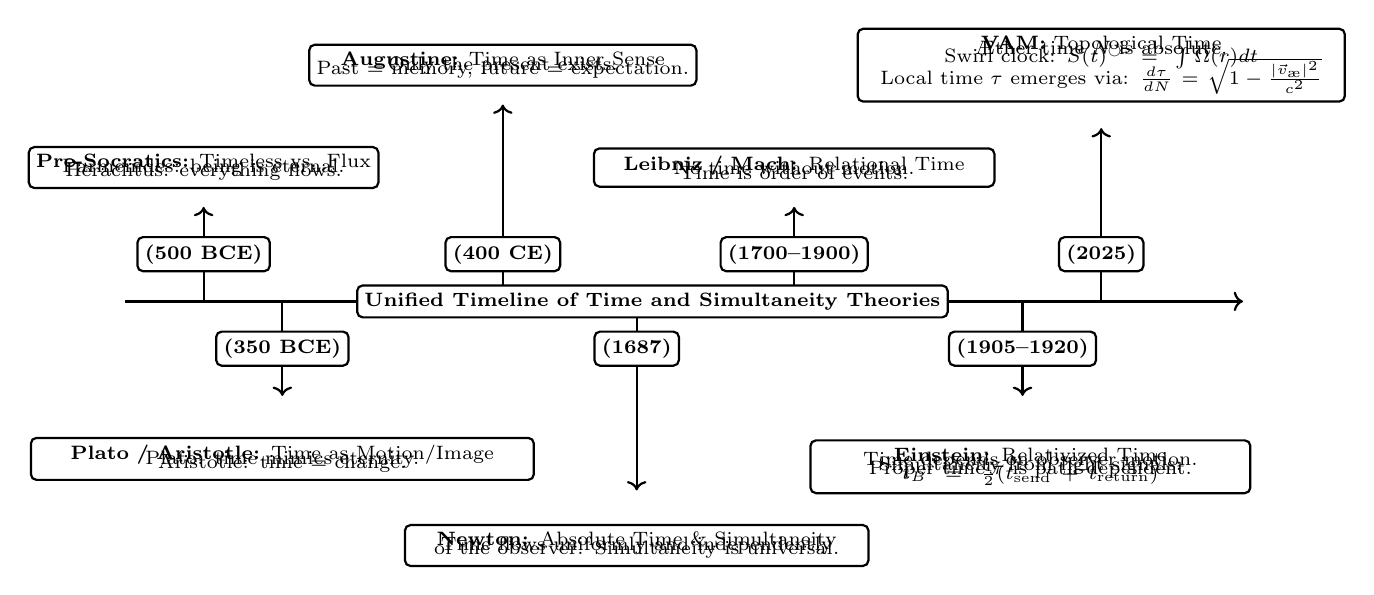
\begin{tikzpicture}
\scriptsize
% Timeline base
\draw[->, thick] (-1,0) -- (13.2,0);

% Arrows above timeline (short, as requested)
\draw[->, thick] (0,0) -- (0,1.2);       % Pre-Socratics
\draw[->, thick] (3.8,0) -- (3.8,2.5);   % Augustine
\draw[->, thick] (7.5,0) -- (7.5,1.2);   % Einstein
\draw[->, thick] (11.4,0) -- (11.4,2.2); % VAM

% Arrows below timeline (short, as requested)
\draw[->, thick] (1.0,0) -- (1.0,-1.2);     % Plato/Aristotle
\draw[->, thick] (5.5,0) -- (5.5,-2.4);     % Newton
\draw[->, thick] (10.4,0) -- (10.4,-1.2);     % Leibniz/Mach

    %--- Root title cards (above timeline) ---
\node[draw, thick, rounded corners=2pt, fill=white, align=center, font=\bfseries ] at (0, .6)   {(500 BCE)};
\node[draw, thick, rounded corners=2pt, fill=white, align=center, font=\bfseries ] at (3.8, .6) {(400 CE)};
\node[draw, thick, rounded corners=2pt, fill=white, align=center, font=\bfseries ] at (7.5, .6) {(1700--1900)};
\node[draw, thick, rounded corners=2pt, fill=white, align=center, font=\bfseries ] at (11.4, .6){(2025)};

%--- Root title cards (below timeline) ---
\node[draw, thick, rounded corners=2pt, fill=white, align=center, font=\bfseries ] at (1.0,- .6) {(350 BCE)};
\node[draw, thick, rounded corners=2pt, fill=white, align=center, font=\bfseries ] at (5.5,- .6) {(1687)};
\node[draw, thick, rounded corners=2pt, fill=white, align=center, font=\bfseries ] at (10.4,- .6) {(1905--1920)};

    % Timeline label
\node[draw, thick, fill=white, rounded corners=2pt, font=\scriptsize] at (5.7,0.0) {\textbf{Unified Timeline of Time and Simultaneity Theories}};

% --- Pre-Socratics ---
\node[draw, rounded corners=2pt, thick, align=center, fill=white] at (0,1.7) {
\textbf{Pre-Socratics:} Timeless vs. Flux \\[-0.8em]
Parmenides: being is eternal. \\[-0.8em]
Heraclitus: everything flows.
};

% --- Augustine ---
\node[draw, rounded corners=2pt, thick, align=center, fill=white] at (3.8,3.0) {
\textbf{Augustine:} Time as Inner Sense \\[-0.8em]
Only the present exists. \\[-0.8em]
Past = memory, future = expectation.
};

% --- Leibniz / Mach ---
\node[draw, rounded corners=2pt, thick, align=center, fill=white, text width=4.9cm] at (7.5,1.7) {
\textbf{Leibniz / Mach:} Relational Time \\[-0.8em]
No time without motion. \\[-0.8em]
Time is order of events.
};
% --- VAM (modern) ---
\node[draw, rounded corners=2pt, thick, align=center, fill=white, text width=6.0cm] at (11.4,3.0) {
\textbf{VAM:} Topological Time \\[-0.8em]
Æther time $N$ is absolute. \\[-0.6em]
Swirl clock: $S(t)^\circlearrowleft = \int \Omega(r) dt$ \\[-0.6em]
Local time $\tau$ emerges via: $ \frac{d\tau}{dN} = \sqrt{1 - \frac{|\vec{v}_\text{\ae}|^2}{c^2}}$

};


% --- Plato / Aristotle ---
\node[draw, rounded corners=2pt, thick, align=center, fill=white, text width=6.2cm] at (1.0,-2) {
\textbf{Plato / Aristotle:} Time as Motion/Image \\[-0.8em]
Plato: time mimics eternity. \\[-0.8em]
Aristotle: time = change.
};



% --- Einstein ---
\node[draw, rounded corners=2pt, thick, align=center, fill=white, text width=5.4cm] at (10.5,-2.1) {
\textbf{Einstein:} Relativized Time \\[-0.8em]
Time depends on observer motion. \\[-0.8em]
Simultaneity from light signals: \\[-0.8em]
Proper time $\tau$ is path-dependent.\\[-0.8em]
$t_B = \frac{1}{2}(t_{\text{send}} + t_{\text{return}})$
};

% --- Newton ---
\node[draw, rounded corners=2pt, thick, align=center, fill=white, text width=5.7cm] at (5.5,-3.1) {
\textbf{Newton:} Absolute Time \& Simultaneity \\[-0.8em]
Time flows uniformly and independently \\[-0.8em]
of the observer. Simultaneity is universal.
};

\end{tikzpicture}
\captionof{figure}{Fused history of time and simultaneity: from early philosophical views and Newton’s absolutes to Einstein’s relativistic structure and VAM’s layered, swirl-based temporality.}
\end{center}

\begin{center}
\footnotesize
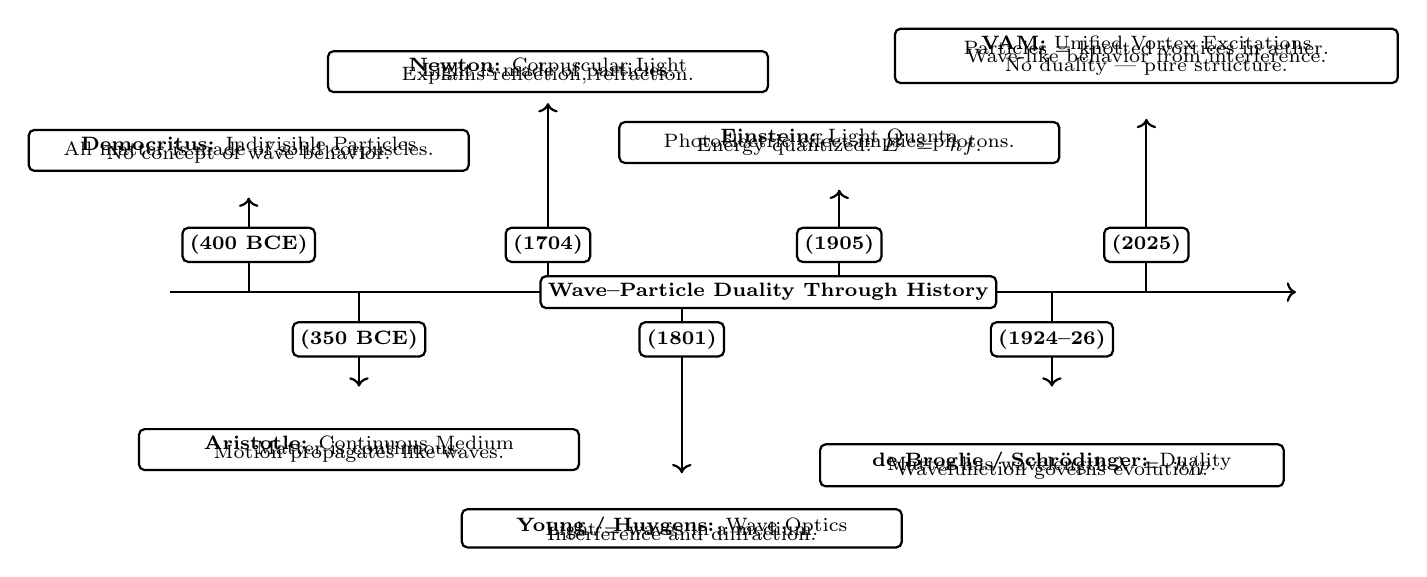
\begin{tikzpicture}
\scriptsize

% Timeline base
\draw[->, thick] (-1,0) -- (13.3,0);

% Arrows above timeline
\draw[->, thick] (0,0) -- (0,1.2);       % Democritus
\draw[->, thick] (3.8,0) -- (3.8,2.4);   % Newton
\draw[->, thick] (7.5,0) -- (7.5,1.3);   % Einstein
\draw[->, thick] (11.4,0) -- (11.4,2.2); % VAM

% Arrows below timeline
\draw[->, thick] (1.4,0) -- (1.4,-1.2);     % Aristotle
\draw[->, thick] (5.5,0) -- (5.5,-2.3);     % Young/Huygens
\draw[->, thick] (10.2,0) -- (10.2,-1.2);   % de Broglie

% --- Date labels ---
\node[draw, thick, rounded corners=2pt, fill=white, align=center, font=\bfseries ] at (0, .6)   {(400 BCE)};
\node[draw, thick, rounded corners=2pt, fill=white, align=center, font=\bfseries ] at (3.8, .6) {(1704)};
\node[draw, thick, rounded corners=2pt, fill=white, align=center, font=\bfseries ] at (7.5, .6) {(1905)};
\node[draw, thick, rounded corners=2pt, fill=white, align=center, font=\bfseries ] at (11.4, .6){(2025)};

\node[draw, thick, rounded corners=2pt, fill=white, align=center, font=\bfseries ] at (1.4,- .6) {(350 BCE)};
\node[draw, thick, rounded corners=2pt, fill=white, align=center, font=\bfseries ] at (5.5,- .6) {(1801)};
\node[draw, thick, rounded corners=2pt, fill=white, align=center, font=\bfseries ] at (10.2,- .6) {(1924--26)};

% Timeline label
\node[draw, thick, fill=white, rounded corners=2pt, font=\scriptsize] at (6.6,0.0) {\textbf{Wave–Particle Duality Through History}};

% --- Democritus ---
\node[draw, rounded corners=2pt, thick, align=center, fill=white, text width=5.4cm] at (0,1.8) {
\textbf{Democritus:} Indivisible Particles \\[-0.8em]
All matter is made of solid corpuscles. \\[-0.8em]
No concept of wave behavior.
};

% --- Newton ---
\node[draw, rounded corners=2pt, thick, align=center, fill=white, text width=5.4cm] at (3.8,2.8) {
\textbf{Newton:} Corpuscular Light \\[-0.8em]
Light is made of particles. \\[-0.8em]
Explains reflection, refraction.
};

% --- Einstein ---
\node[draw, rounded corners=2pt, thick, align=center, fill=white, text width=5.4cm] at (7.5,1.9) {
\textbf{Einstein:} Light Quanta \\[-0.8em]
Photoelectric effect implies photons. \\[-0.8em]
Energy quantized: \( E = hf \).
};

% --- VAM ---
\node[draw, rounded corners=2pt, thick, align=center, fill=white, text width=6.2cm] at (11.4,3.0) {
\textbf{VAM:} Unified Vortex Excitations \\[-0.8em]
Particles = knotted vortices in æther. \\[-0.6em]
Wave-like behavior from interference. \\[-0.6em]
No duality — pure structure.
};

% --- Aristotle ---
\node[draw, rounded corners=2pt, thick, align=center, fill=white, text width=5.4cm] at (1.4,-2.0) {
\textbf{Aristotle:} Continuous Medium \\[-0.8em]
Matter is continuous. \\[-0.8em]
Motion propagates like waves.
};

% --- Young / Huygens ---
\node[draw, rounded corners=2pt, thick, align=center, fill=white, text width=5.4cm] at (5.5,-3.0) {
\textbf{Young / Huygens:} Wave Optics \\[-0.8em]
Light = waves in a medium. \\[-0.8em]
Interference and diffraction.
};

% --- de Broglie / Schrödinger ---
\node[draw, rounded corners=2pt, thick, align=center, fill=white, text width=5.7cm] at (10.2,-2.2) {
\textbf{de Broglie / Schrödinger:} Duality \\[-0.8em]
Matter has wavelength \( \lambda = h/p \). \\[-0.8em]
Wavefunction governs evolution.
};

\end{tikzpicture}
\captionof{figure}{Development of wave–particle duality: from atomistic corpuscles and wave optics, through quantum superposition, to VAM’s unified vortex excitation model.}
\end{center}
\sout{}
    \begin{center}
        \footnotesize
        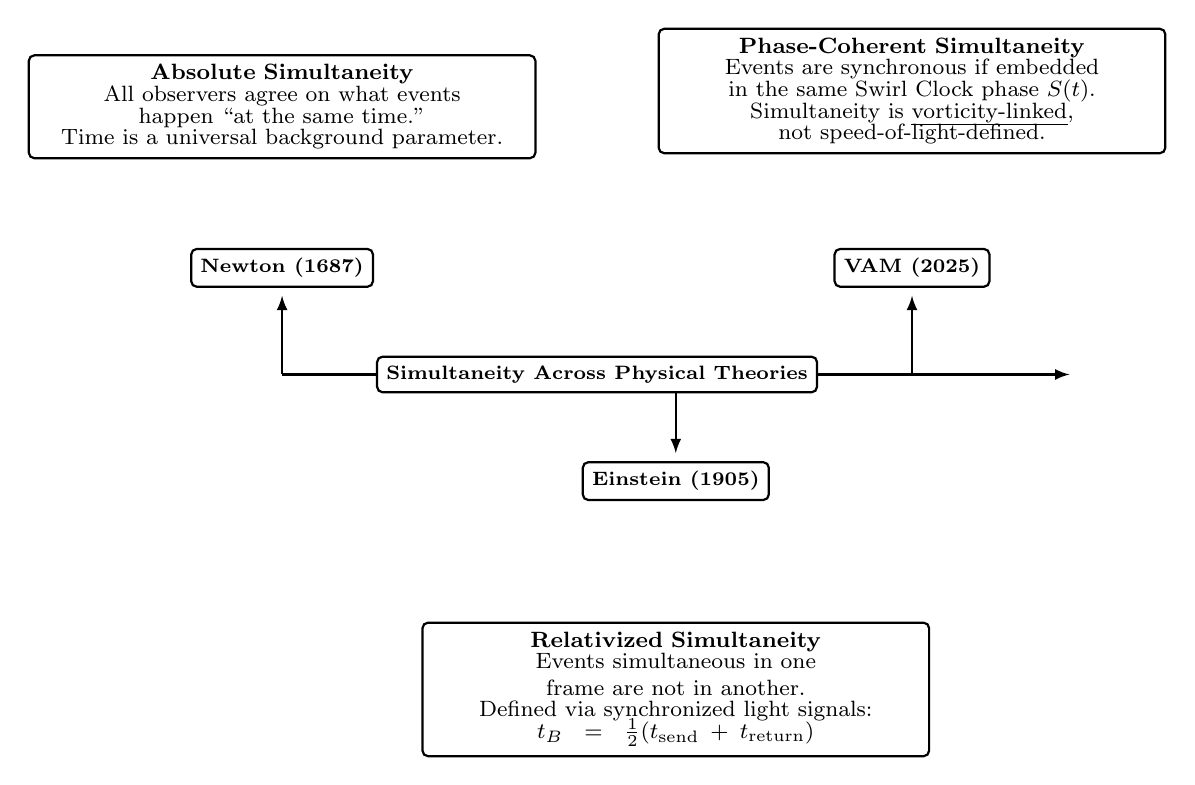
\begin{tikzpicture}[node distance=3.5cm, every node/.style={font=\footnotesize}, >=latex]

    % Timeline (adjusted)
            \draw[->, thick] (0,0) -- (10,0);

    % Newton (left)
            \node[draw, rounded corners=2pt, thick, align=center, fill=white, text width=6.2cm]  at (0,3.4) {
                \textbf{Absolute Simultaneity} \\[-0.2em]
                All observers agree on what events \\[-0.2em]
                happen ``at the same time.'' \\[-0.2em]
                Time is a universal background parameter.
            };
            \draw[->, thick] (0,0.0) -- (0,1.0);
            \node[above=1.1cm, draw, thick, fill=white, rounded corners=2pt, font=\scriptsize] at (0,0) {\textbf{Newton (1687)}};

    % Einstein (center)
            \node[draw, rounded corners=2pt, thick, align=center, fill=white, text width=6.2cm]  at (5,-4.0) {
                \textbf{Relativized Simultaneity} \\[-0.2em]
                Events simultaneous in one frame are not in another. \\[-0.2em]
                Defined via synchronized light signals: \\[-0.2em]
                $t_B = \frac{1}{2}(t_{\text{send}} + t_{\text{return}})$
            };
            \draw[->, thick] (5,0.0) -- (5,-1.0);
            \node[below=1.1cm, draw, thick, fill=white, rounded corners=2pt, font=\scriptsize]  at (5,0) {\textbf{Einstein (1905)}};

    % VAM (right)
            \node[draw, rounded corners=2pt, thick, align=center, fill=white, text width=6.2cm]  at (8,3.6) {
                \textbf{Phase-Coherent Simultaneity} \\[-0.2em]
                Events are synchronous if embedded \\[-0.2em]
                in the same Swirl Clock phase $S(t)$. \\[-0.2em]
                Simultaneity is \emph{vorticity-linked}, \\[-0.2em]
                not speed-of-light-defined.
            };
            \draw[->, thick] (8,0.0) -- (8,1.0);
            \node[above=1.1cm, draw, thick, fill=white, rounded corners=2pt, font=\scriptsize] at (8,0) {\textbf{VAM (2025)}};

    % Timeline label above axis in box (higher)
            \node[draw, thick, fill=white, rounded corners=2pt, font=\scriptsize] at (4,0.0) {\textbf{Simultaneity Across Physical Theories}};

        \end{tikzpicture}
        \captionof{figure}{Three conceptions of simultaneity: Newton’s universal now, Einstein’s light-signal-based frame dependence, and VAM’s internal phase coherence across vortex structures.}
    \end{center}


    \vspace{-1em}


\begin{center}
\footnotesize
\begin{tikzpicture}[node distance=3.5cm, every node/.style={font=\footnotesize}, >=latex]



% Timeline base
\draw[->, thick] (-1,0) -- (13.2,0);

% Arrows above timeline (short, as requested)
\draw[->, thick] (0,0) -- (0,1.2);       % Pre-Socratics
\draw[->, thick] (3.8,0) -- (3.8,2.5);   % Augustine
\draw[->, thick] (7.5,0) -- (7.5,1.2);   % Einstein
\draw[->, thick] (11.4,0) -- (11.4,3.0); % VAM

% Arrows below timeline (short, as requested)
\draw[->, thick] (1.0,0) -- (1.0,-1.2);     % Plato/Aristotle
\draw[->, thick] (5.5,0) -- (5.5,-2.4);     % Newton
\draw[->, thick] (10.4,0) -- (10.4,-1.2);     % Leibniz/Mach

    %--- Root title cards (above timeline) ---
\node[draw, thick, rounded corners=2pt, fill=white, align=center, font=\bfseries ] at (0, .6)   {(500 BCE)};
\node[draw, thick, rounded corners=2pt, fill=white, align=center, font=\bfseries ] at (3.8, .6) {(400 CE)};
\node[draw, thick, rounded corners=2pt, fill=white, align=center, font=\bfseries ] at (7.5, .6) {(1700--1900)};
\node[draw, thick, rounded corners=2pt, fill=white, align=center, font=\bfseries ] at (11.4, .6){(2025)};

%--- Root title cards (below timeline) ---
\node[draw, thick, rounded corners=2pt, fill=white, align=center, font=\bfseries ] at (1.0,- .6) {(350 BCE)};
\node[draw, thick, rounded corners=2pt, fill=white, align=center, font=\bfseries ] at (5.5,- .6) {(1687)};
\node[draw, thick, rounded corners=2pt, fill=white, align=center, font=\bfseries ] at (10.4,- .6) {(1905--1920)};

% Label (centered box)
\node[draw, thick, fill=white, rounded corners=2pt, font=\scriptsize] at (5.7,0.0) {\textbf{Ontology of Time in Western Science}};

% Ancient Greek: Parmenides / Heraclitus
\node[draw, rounded corners=2pt, thick, align=center, fill=white, text width=5cm] at (0,2.6) {
\textbf{Timeless vs. Flux (ca. 500 BCE)} \\[-0.2em]
Parmenides: timeless being. \\[-0.2em]
Heraclitus: constant change (\textit{panta rhei}).
};

\node[above=1.6cm, draw, thick, fill=white, rounded corners=2pt, font=\scriptsize] at (0,0) {\textbf{Pre-Socratics}};

% Plato / Aristotle
\node[draw, rounded corners=2pt, thick, align=center, fill=white, text width=5cm] at (2.2,-3.0) {
\textbf{Time as Motion/Image (ca. 350 BCE)} \\[-0.2em]
Plato: moving image of eternity. \\[-0.2em]
Aristotle: number of change.
};

\node[below=2.0cm, draw, thick, fill=white, rounded corners=2pt, font=\scriptsize] at (2.2,0) {\textbf{Plato / Aristotle}};

% Augustine
\node[draw, rounded corners=2pt, thick, align=center, fill=white, text width=5cm] at (4.3,2.8) {
\textbf{Time as Inner Sense (400 CE)} \\[-0.2em]
Past = memory, future = anticipation. \\[-0.2em]
Only the present is real.
};

\node[above=1.8cm, draw, thick, fill=white, rounded corners=2pt, font=\scriptsize] at (4.3,0) {\textbf{Augustine}};

% Newton
\node[draw, rounded corners=2pt, thick, align=center, fill=white, text width=5cm] at (6.2,-3.2) {
\textbf{Absolute Time (1687)} \\[-0.2em]
Time flows uniformly, \\[-0.2em]
independent of events.
};

\node[below=2.0cm, draw, thick, fill=white, rounded corners=2pt, font=\scriptsize] at (6.2,0) {\textbf{Newton}};

% Relationalists: Leibniz / Mach
\node[draw, rounded corners=2pt, thick, align=center, fill=white, text width=5cm] at (8.0,2.8) {
\textbf{Relational Time (1700–1900)} \\[-0.2em]
Time = order of events. \\[-0.2em]
No time without change.
};

\node[above=1.8cm, draw, thick, fill=white, rounded corners=2pt, font=\scriptsize] at (8.0,0) {\textbf{Leibniz / Mach}};

% Einstein
\node[draw, rounded corners=2pt, thick, align=center, fill=white, text width=5cm] at (10.0,-3.0) {
\textbf{Relative & Curved Time (1905–1915)} \\[-0.2em]
Time depends on observer motion. \\[-0.2em]
Becomes curved in gravity.
};

\node[below=2.0cm, draw, thick, fill=white, rounded corners=2pt, font=\scriptsize] at (10.0,0) {\textbf{Einstein}};

% VAM
\node[draw, rounded corners=2pt, thick, align=center, fill=white, text width=5cm] at (12.2,2.8) {
\textbf{Layered Time (2025)} \\[-0.2em]
Global time \( \mathcal{N} \), \\[-0.2em]
Proper time \( \tau \), \\[-0.2em]
Swirl phase \( S(t) = \int \Omega dt \).
};

\node[above=1.8cm, draw, thick, fill=white, rounded corners=2pt, font=\scriptsize] at (12.2,0) {\textbf{VAM}};

\end{tikzpicture}
\captionof{figure}{Historical evolution of temporal ontology: from pre-Socratic polarity to Einstein's spacetime and the layered temporality of the Vortex Æther Model.}
\end{center}


\begin{center}
\footnotesize
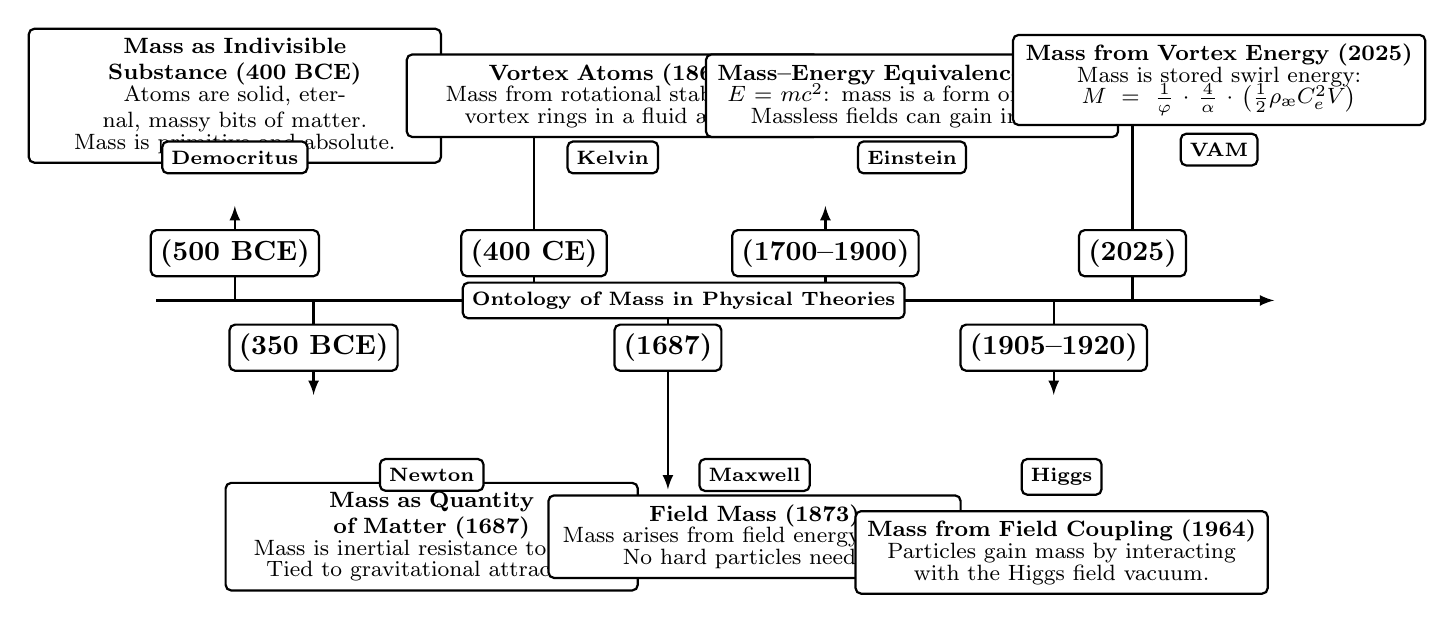
\begin{tikzpicture}[node distance=3.5cm, every node/.style={font=\footnotesize}, >=latex]


% Timeline base
\draw[->, thick] (-1,0) -- (13.2,0);

% Arrows above timeline (short, as requested)
\draw[->, thick] (0,0) -- (0,1.2);       % Pre-Socratics
\draw[->, thick] (3.8,0) -- (3.8,2.5);   % Augustine
\draw[->, thick] (7.5,0) -- (7.5,1.2);   % Einstein
\draw[->, thick] (11.4,0) -- (11.4,3.0); % VAM

% Arrows below timeline (short, as requested)
\draw[->, thick] (1.0,0) -- (1.0,-1.2);     % Plato/Aristotle
\draw[->, thick] (5.5,0) -- (5.5,-2.4);     % Newton
\draw[->, thick] (10.4,0) -- (10.4,-1.2);     % Leibniz/Mach

    %--- Root title cards (above timeline) ---
\node[draw, thick, rounded corners=2pt, fill=white, align=center, font=\bfseries ] at (0, .6)   {(500 BCE)};
\node[draw, thick, rounded corners=2pt, fill=white, align=center, font=\bfseries ] at (3.8, .6) {(400 CE)};
\node[draw, thick, rounded corners=2pt, fill=white, align=center, font=\bfseries ] at (7.5, .6) {(1700--1900)};
\node[draw, thick, rounded corners=2pt, fill=white, align=center, font=\bfseries ] at (11.4, .6){(2025)};

%--- Root title cards (below timeline) ---
\node[draw, thick, rounded corners=2pt, fill=white, align=center, font=\bfseries ] at (1.0,- .6) {(350 BCE)};
\node[draw, thick, rounded corners=2pt, fill=white, align=center, font=\bfseries ] at (5.5,- .6) {(1687)};
\node[draw, thick, rounded corners=2pt, fill=white, align=center, font=\bfseries ] at (10.4,- .6) {(1905--1920)};

% Label
\node[draw, thick, fill=white, rounded corners=2pt, font=\scriptsize] at (5.7,0.0) {\textbf{Ontology of Mass in Physical Theories}};

% Democritus (left)
\node[draw, rounded corners=2pt, thick, align=center, fill=white, text width=5cm] at (0,2.6) {
\textbf{Mass as Indivisible Substance (400 BCE)} \\[-0.2em]
Atoms are solid, eternal, massy bits of matter. \\[-0.2em]
Mass is primitive and absolute.
};

\node[above=1.6cm, draw, thick, fill=white, rounded corners=2pt, font=\scriptsize] at (0,0) {\textbf{Democritus}};

% Newton (below)
\node[draw, rounded corners=2pt, thick, align=center, fill=white, text width=5cm] at (2.5,-3.0) {
\textbf{Mass as Quantity of Matter (1687)} \\[-0.2em]
Mass is inertial resistance to force. \\[-0.2em]
Tied to gravitational attraction.
};

\node[below=2.0cm, draw, thick, fill=white, rounded corners=2pt, font=\scriptsize] at (2.5,0) {\textbf{Newton}};

% Kelvin (top)
\node[draw, rounded corners=2pt, thick, align=center, fill=white, text width=5cm] at (4.8,2.6) {
\textbf{Vortex Atoms (1867)} \\[-0.2em]
Mass from rotational stability of \\[-0.2em]
vortex rings in a fluid æther.
};

\node[above=1.6cm, draw, thick, fill=white, rounded corners=2pt, font=\scriptsize] at (4.8,0) {\textbf{Kelvin}};

% Maxwell (bottom)
\node[draw, rounded corners=2pt, thick, align=center, fill=white, text width=5cm] at (6.6,-3.0) {
\textbf{Field Mass (1873)} \\[-0.2em]
Mass arises from field energy density. \\[-0.2em]
No hard particles needed.
};

\node[below=2.0cm, draw, thick, fill=white, rounded corners=2pt, font=\scriptsize] at (6.6,0) {\textbf{Maxwell}};

% Einstein (top)
\node[draw, rounded corners=2pt, thick, align=center, fill=white, text width=5cm] at (8.6,2.6) {
\textbf{Mass–Energy Equivalence (1905)} \\[-0.2em]
\( E = mc^2 \): mass is a form of energy. \\[-0.2em]
Massless fields can gain inertia.
};

\node[above=1.6cm, draw, thick, fill=white, rounded corners=2pt, font=\scriptsize] at (8.6,0) {\textbf{Einstein}};

% Higgs (bottom)
\node[draw, rounded corners=2pt, thick, align=center, fill=white, text width=5cm] at (10.5,-3.2) {
\textbf{Mass from Field Coupling (1964)} \\[-0.2em]
Particles gain mass by interacting \\[-0.2em]
with the Higgs field vacuum.
};

\node[below=2.0cm, draw, thick, fill=white, rounded corners=2pt, font=\scriptsize] at (10.5,0) {\textbf{Higgs}};

% VAM (top right)
\node[draw, rounded corners=2pt, thick, align=center, fill=white, text width=5cm] at (12.5,2.8) {
\textbf{Mass from Vortex Energy (2025)} \\[-0.2em]
Mass is stored swirl energy: \\[-0.2em]
\( M = \frac{1}{\varphi} \cdot \frac{4}{\alpha} \cdot \left( \frac{1}{2} \rho_\text{\ae} C_e^2 V \right) \)
};

\node[above=1.7cm, draw, thick, fill=white, rounded corners=2pt, font=\scriptsize] at (12.5,0) {\textbf{VAM}};

\end{tikzpicture}
\captionof{figure}{Historical evolution of mass ontology: from indivisible substance to field energy and finally to vortex-stored rotational energy in the ætheric continuum of VAM.}
\end{center}


\section*{Final Reflection: Æther Past and Future}

    These appendices trace a conceptual lineage—beginning with Maxwell's mechanical æther as a carrier of field stresses, evolving through Kelvin's vision of atoms as knotted vortex rings, and reformulated by Einstein into a geometric substrate underlying spacetime itself. Each step preserved the core intuition: that empty space is not truly empty, but possesses structure, energy, and dynamical influence.

    The Vortex Æther Model (VAM) completes this lineage by merging the fluid and field paradigms into a unified topological framework. In VAM, the æther is no longer an abstract scaffolding or discarded relic, but a physically real medium: incompressible, inviscid, and threaded with quantized vorticity. Mass arises from rotational energy; gravity from swirl-induced pressure gradients; time from the internal phase of topological knots.

    Where previous æther models lacked formal consistency or empirical validation, VAM draws on modern tools—fluid dynamics, knot theory, Hamiltonian flows, and high-precision measurement—to revisit the æther hypothesis with scientific rigor and predictive power.

    Einstein redefined the æther without abandoning it. VAM takes the next step—restoring motion, structure, and causality to the medium beneath all physical law.



    \bibliographystyle{unsrt}
    \bibliography{VAM-0-From_Einstein_to_the_Vortex_Fluid_paradigm}
\end{document}